% Chapter Template

\chapter{Background} % Main chapter title

\label{Chapter2} % For referencing the chapter elsewhere, use \ref{Chapter1} 

One of the requirements of this thesis was the ability to work with linked data. As well as the React framework, because of high usage of that framework in other projects that are developed by \groupname. So now in this chapter, introduce the technologies that are related to this thesis.

%----------------------------------------------------------------------------------------
%	SECTION 1
%----------------------------------------------------------------------------------------

\section{Resource Description Framework}

Resource Description Framework \parencite{Guha+Brickey+McBride} is a general description framework for describing informations provided by web sources. This framework creates a basis for the semantic web. Representation of the RDF can be as a graph or dataset. 

In graph representation, data are a set of RDF triplets. Each triplet consists of three components - subject, predicate, and object. Subject and object are nodes and predicate is an edge of the graph. Triplet in official terminology express some facts about the source. A claim consists of three pieces that together create a sentence: subject --> predicate --> object.  Within this statement, the source is a subject identified by URI (or IRI), the property is a predicate (what we say about the source), and value is an object. Predicates that we used for describing a source come from so-called schemas – that are
vocabularies or ontologies. Examples can be \cite{DC} or \cite{foaf} metadata standards. RDF syntax has various type of formats that are called serialization formats. Among these formats are for example Turtle, N-Quads, N-Triplets, or JSON-LD.\parencite{JSON-LD}

An RDF dataset is a set of RDF graphs. This set can consist of:
\begin{itemize}
\item default graph - exactly one RDF graph that does not have a name and may be empty
\item named graphs - a pair of RDF graph and IRI or blank node
\end{itemize}


%----------------------------------------------------------------------------------------
%	SECTION 2
%----------------------------------------------------------------------------------------

\section{Linked Data}

To understand what is Linked Data, you do not need any experience with web programming, just a basic knowledge of HTTP, URI, and IRI. The concept of Linked Data \parencite{Bizare+heath+Berners-Lee,Heath+Bizer} is following. Firstly, lest start what data are. Data are sets of values consisting of pieces of information. Problem with these data is that they do not carry any context about the information they represent. Imagine this example, two different data objects both objects have a property called 'name' with some value. That property represents some name, but without any further knowledge, that name representation can have a different meaning in each object.

On the other hand, Linked Data help to solve the problem by describing and interconnecting data by shared vocabularies. By packaging a data in the way that they express what kind of data they represent,  you will receive a Linked Data. With all of this, there are still two main problems. First is what format use for Linked Data. There are lots of formats, for example, JSON, RDFa, XML, CSV, HTML, etc. The second problem is how we can link the pieces of data together. Most common and easiest way to express data is on the key-value pair. 

%----------------------------------------------------------------------------------------
%	SECTION 3
%----------------------------------------------------------------------------------------

\section{JSON-LD}
JSON-LD is a format based on JSON format. JSON format is easy to use in a web application because it is readily convertible to JavaScript object, which represents data in a web application


JSON-LD is an RDF syntax for describing linked data using JSON format. \parencite{JSON-LD} JSON-LD is both JSON document and RDF document \parencite{RDF_doc}, but it has some differences with RDF. First, JSON-LD properties can be URIs (or IRIs) or blank nodes whereas in RDF properties must be URIs (or IRIs). That means that JSON-LD can serialize RDF data-sets. The other direction is not possible. Second, JSON-LD object lists are part of data model whereas RDF objects are part of the vocabulary. The last one, RDF values are either literals or language-tagged strings whereas JSON-LD also supports JavaScript native types, which are numbers, booleans, and strings.

\begin{figure}[th]
    \centering
    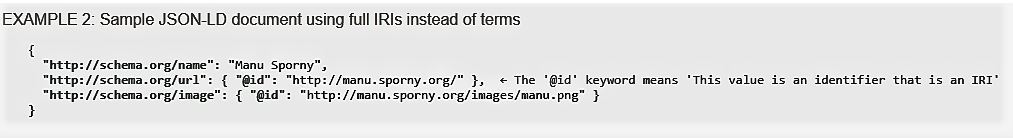
\includegraphics[width=\textwidth]{JSON-LD_example}
    \decoRule
    \caption[JSON-LD document]{Example of JSON-LD document}
    \label{fig:JSON-LD_document}
 \end{figure}

%----------------------------------------------------------------------------------------
%	SECTION 4
%----------------------------------------------------------------------------------------

\section{React, Redux}

React \parencite{react} is a JavaScript UI framework developed and maintained by Facebook. Its one of the most used framework because it's easy to learn and because of its performance efficiency. If
you are familiar with the MVC model\parencite{MVC}, React is only the view part. Redux \parencite{Redux} is completely independent on React. Redux is a state container for JavaScript. This means, that Redux is just a framework for managing the state of your web applications. It evolves from Flux \parencite{Flux} framework but does not take Flux complexity.

%----------------------------------------------------------------------------------------
%	SECTION 5
%----------------------------------------------------------------------------------------

\section{React virtualized select and React select}

\cite{react-virtualized-select} and \cite{react-select} as the name suggests, are both
React components. Both components are almost same.  As the Brian Vaughn says: 
"react-select-virtualized works just like react-select". The only difference between them 
is that the first component is able to render large list more efficiently. This was 
achieved by a special way of rendering options. In a nutshell, the drop-down menu is 
rendered only with a minimum required amount of options that are in focus (visible in 
the drop-down menu). A detailed description of this process will be described later on.

%----------------------------------------------------------------------------------------